\documentclass{beamer}

\pdfmapfile{+sansmathaccent.map}


\mode<presentation>
{
  \usetheme{Warsaw} % or try Darmstadt, Madrid, Warsaw, Rochester, CambridgeUS, ...
  \usecolortheme{seahorse} % or try seahorse, beaver, crane, wolverine, ...
  \usefonttheme{serif}  % or try serif, structurebold, ...
  \setbeamertemplate{navigation symbols}{}
  \setbeamertemplate{caption}[numbered]
} 


%%%%%%%%%%%%%%%%%%%%%%%%%%%%
% itemize settings

\definecolor{mypink}{RGB}{255, 150, 150}
\definecolor{myblue}{RGB}{150, 150, 255}
\definecolor{mygray}{gray}{0.8}

\setbeamertemplate{itemize items}[default]

\setbeamertemplate{itemize item}{\color{mypink}$\blacksquare$}
\setbeamertemplate{itemize subitem}{\color{myblue}$\blacktriangleright$}
\setbeamertemplate{itemize subsubitem}{\color{mygray}$\blacksquare$}

%%%%%%%%%%%%%%%%%%%%%%%%%%%%
% block settings

\setbeamercolor{block title}{bg=red!30,fg=black}


%%%%%%%%%%%%%%%%%%%%%%%%%%%%
% URL settings
\hypersetup{
    colorlinks=true,
    linkcolor=blue,
    filecolor=blue,      
    urlcolor=blue,
}

%%%%%%%%%%%%%%%%%%%%%%%%%%

\renewcommand{\familydefault}{\rmdefault}

\usepackage{amsmath}
\usepackage{mathtools}

\DeclareMathOperator*{\argmin}{arg\,min}

\usepackage{subcaption}




%%%%%%%%%%%%%%%%%%%%%%%%%%%%
% code settings

\usepackage{listings}
\usepackage{color}
\definecolor{mygreen}{rgb}{0,0.6,0}
\definecolor{mygray}{rgb}{0.5,0.5,0.5}
\definecolor{mymauve}{rgb}{0.58,0,0.82}
\lstset{ 
  backgroundcolor=\color{white},   % choose the background color; you must add \usepackage{color} or \usepackage{xcolor}; should come as last argument
  basicstyle=\footnotesize,        % the size of the fonts that are used for the code
  breakatwhitespace=false,         % sets if automatic breaks should only happen at whitespace
  breaklines=true,                 % sets automatic line breaking
  captionpos=b,                    % sets the caption-position to bottom
  commentstyle=\color{mygreen},    % comment style
  deletekeywords={...},            % if you want to delete keywords from the given language
  escapeinside={\%*}{*)},          % if you want to add LaTeX within your code
  extendedchars=true,              % lets you use non-ASCII characters; for 8-bits encodings only, does not work with UTF-8
  firstnumber=0000,                % start line enumeration with line 0000
  frame=single,	                   % adds a frame around the code
  keepspaces=true,                 % keeps spaces in text, useful for keeping indentation of code (possibly needs columns=flexible)
  keywordstyle=\color{blue},       % keyword style
  language=Octave,                 % the language of the code
  morekeywords={*,...},            % if you want to add more keywords to the set
  numbers=left,                    % where to put the line-numbers; possible values are (none, left, right)
  numbersep=5pt,                   % how far the line-numbers are from the code
  numberstyle=\tiny\color{mygray}, % the style that is used for the line-numbers
  rulecolor=\color{black},         % if not set, the frame-color may be changed on line-breaks within not-black text (e.g. comments (green here))
  showspaces=false,                % show spaces everywhere adding particular underscores; it overrides 'showstringspaces'
  showstringspaces=false,          % underline spaces within strings only
  showtabs=false,                  % show tabs within strings adding particular underscores
  stepnumber=2,                    % the step between two line-numbers. If it's 1, each line will be numbered
  stringstyle=\color{mymauve},     % string literal style
  tabsize=2,	                   % sets default tabsize to 2 spaces
  title=\lstname                   % show the filename of files included with \lstinputlisting; also try caption instead of title
}

%%%%%%%%%%%%%%%%%%%%%%%%%%%%
% tikz settings

\usepackage{tikz}
\tikzset{every picture/.style={line width=0.75pt}}


\title{Control with QP and SOCP}
\subtitle{Contact-aware Control, Lecture 8}
\author{by Sergei Savin}
\centering
\date{Fall 2020}



\begin{document}
\maketitle


\begin{frame}{Content}

\begin{itemize}
\item Quadratic programming
\begin{itemize}
\item Special case with an analytic solution
\item Example
\item Example - solution using quadprog
\item Example - solution using CVX
\item Application
\item What it can’t do
\end{itemize}
\item Second-order cone programming
\item Friction cone and SOCP
\begin{itemize}
\item Formulation
\item Application
\end{itemize}
\item Read more
\end{itemize}

\end{frame}



\begin{frame}{Quadratic programming}
% \framesubtitle{Part 1}
\begin{flushleft}

There are special cases of optimization problems that can be solved numerically very efficiently. One of those is \emph{quadratic programming}.

\bigskip

General form of a quadratic program (QP) is given below:

%
\begin{equation}
\begin{aligned}
& \underset{\mathbf{x}}{\text{minimize}}
& & \mathbf{x}^\top \mathbf{H} \mathbf{x} + \mathbf{f}^\top\mathbf{x}, \\
& \text{subject to}
& & \begin{cases}
    \mathbf{A}\mathbf{x} \leq \mathbf{b}, \\
    \mathbf{C}\mathbf{x} = \mathbf{d}.
    \end{cases}
\end{aligned}
\end{equation}

where $\mathbf{H}$ is positive-definite and $\mathbf{A}\mathbf{x} \leq \mathbf{b}$ describe a \emph{convex region}.

\end{flushleft}
\end{frame}



\begin{frame}{Quadratic programming}
\framesubtitle{Special case with an analytic solution}
\begin{flushleft}

If there are no inequality constraints: 

\begin{equation}
\begin{aligned}
& \underset{\mathbf{x}}{\text{minimize}}
& & \mathbf{x}^\top \mathbf{H} \mathbf{x} + \mathbf{c}^\top\mathbf{x}, \\
& \text{subject to}
& & \mathbf{A} \mathbf{x} = \mathbf{b}.
\end{aligned}
\end{equation}

a quadratic program can be solved analytically.

\end{flushleft}
\end{frame}



\begin{frame}{Quadratic programming}
\framesubtitle{Example}
\begin{flushleft}

We have the following problem: find such $\mathbf x$ that minimizes $\mathbf x^\top \mathbf M \mathbf x$, while $\mathbf C \mathbf x = \mathbf y$. In other words:

\begin{equation} \label{eq:Example1:1}
\begin{aligned}
& \underset{\mathbf  x}{\text{minimize}}
& & \mathbf x^\top \mathbf M \mathbf x, \\
& \text{subject to}
& & \mathbf C \mathbf x = \mathbf y.
\end{aligned}
\end{equation}

More concrete:

\begin{equation} \label{eq:Example1:2}
\begin{aligned}
& \underset{\mathbf  x}{\text{minimize}}
& & \begin{bmatrix} x_1 & x_2 & x_3 \end{bmatrix}
\begin{bmatrix}  
   1 & 0 & 1 \\
   0 & 5 & 0 \\
   1 & 0 & 3 \\
   \end{bmatrix}
\begin{bmatrix} x_1 \\ x_2 \\ x_3 \end{bmatrix}, \\
& \text{subject to}
& & \begin{bmatrix} 1 & 7 & 2 \end{bmatrix}
\begin{bmatrix} x_1 \\ x_2 \\ x_3 \end{bmatrix}
= 1.
\end{aligned}
\end{equation}

\end{flushleft}
\end{frame}




\begin{frame}{Quadratic programming}
\framesubtitle{Example - solution using quadprog}
\begin{flushleft}

We can use a dedicated solver for this class of problems - \texttt{quadprog} provided by MATLAB. Here is the solution:

\begin{lstlisting}[language=Matlab]
    C_times_v = reshape(dHdt*v, length(v), 1) - reshape(jacobian((0.5*v' * H * v), q), length(v), 1);
\end{lstlisting}

Average solution time is \textbf{0.56} ms

\end{flushleft}
\end{frame}




\begin{frame}{Quadratic programming}
\framesubtitle{Example - solution using CVX}
\begin{flushleft}

Alternatively we can invoke one of the most powerful convex optimization tools with a user-friendly coding style - CVX:

\begin{lstlisting}[language=Matlab]
M = [1 0 1; 0 5 0; 1 0 3];
C = [1 7 2];
y = 1;

cvx_begin
variables x(3);
minimize( x' * M * x );
subject to
    C*x == y;
cvx_end
\end{lstlisting}

\href{http://cvxr.com/cvx/}{Official web page of the CVX package}

\end{flushleft}
\end{frame}






\begin{frame}{Quadratic programming}
\framesubtitle{Application}
\begin{flushleft}

Remember CTC control from the lecture on error dynamics:

\begin{equation}
\begin{cases}
    \bo{v} = \bo{H}(\ddot{\bo{q}}^* + \bo{K}_d\dot{\bo{e}} + \bo{K}_p\bo{e}) + \bo{c} \\
    \bo{T}\bo{u} + \bo{F}^\top \lambda = \bo{v}
\end{cases}
\end{equation}

Assume that $\lambda = [\lambda_1^\top, \ ...  \lambda_m^\top]^\top \in \R^{3m}$, $\lambda_i \in \R^{3}$ and represents a $m$ individual unilateral contact with normal unit-vectors to the contact surface $\bo{n}_i$, and no friction. Then we can write the control law as a solution to the quadratic program:

\begin{equation}
\begin{aligned}
& \underset{\bo{u}, \bo{v}, \lambda_i}{\text{minimize}}
& & \mathbf{u}^\top \mathbf{u}, \\
& \text{subject to}
& & \begin{cases}
    \bo{H}(\ddot{\bo{q}}^* + \bo{K}_d\dot{\bo{e}} + \bo{K}_p\bo{e}) + \bo{c} = \bo{v} \\
    \bo{T}\bo{u} + \sum\limits_{i = 1}^m \bo{F}_i^\top \lambda_i = \bo{v} \\\
    -\bo{n}_i^\top \lambda_i \leq 0
\end{cases}
\end{aligned}
\end{equation}

\end{flushleft}
\end{frame}



\begin{frame}{Quadratic programming}
\framesubtitle{What it can't do}
\begin{flushleft}

Remember friction cone constraints:

\begin{equation}
\label{eq:friction_cone_2}
    || [\tau_1 \ \tau_2]^\top \bo{f} || \leq \mu \bo{n}^\top \bo{f}
\end{equation}

These can't be directly represented in a quadratic program.

\end{flushleft}
\end{frame}



\begin{frame}{Second-order cone programming}
\framesubtitle{General form}
\begin{flushleft}

The general form of a Second-order cone program (SOCP) is:

%
\begin{equation}
\begin{aligned}
& \underset{\mathbf{x}}{\text{minimize}}
& & \mathbf{f}^\top\mathbf{x}, \\
& \text{subject to}
& & \begin{cases}
    ||\mathbf{A}_i\mathbf{x} + \mathbf{b}_i||_2 \leq 
     \mathbf{c}_i^\top \mathbf{x} + d_i, \\
    \mathbf{F}\mathbf{x} = g.
    \end{cases}
\end{aligned}
\end{equation}

QP are a subset of SOCP.
 
\end{flushleft}
\end{frame}



\begin{frame}{Friction cone and SOCP}
% \framesubtitle{O}
\begin{flushleft}

We already saw that a no-friction contact can be represented as a QP. Next we will try to show that friction cone (a more general model) can be represented as a SOPC (a more general optimization problem type).

\begin{figure}
    \centering
    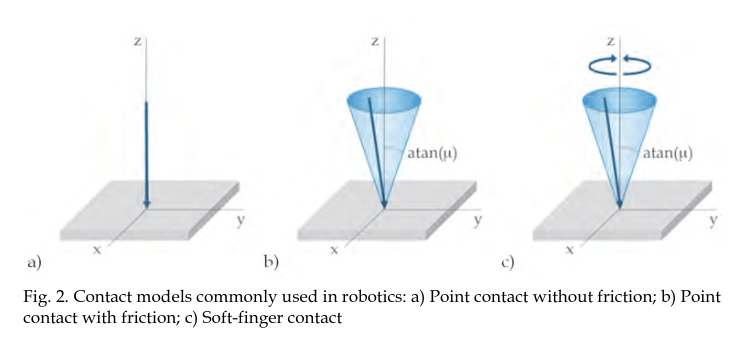
\includegraphics[width= 0.85\linewidth]{fig2.png}
    % \caption{}
    \label{fig:contact}
\end{figure}

\scriptsize{Picture is from \emph{Sancho-Bru, J.L., P\'{e}rez-Gonz\'{a}lez, A., Mora, M.C., L\'{o}n, B.E., Vergara, M., Iserte, J.L., Rodriguez-Cervantes, P.J. and Morales, A., 2011. Towards a realistic and self-contained biomechanical model of the hand. In Theoretical biomechanics. IntechOpen.}}

\end{flushleft}
\end{frame}



\begin{frame}{Friction cone and SOCP}
\framesubtitle{Formulation}
\begin{flushleft}

Coming back to the the friction cone general view:

\begin{equation}
    || [\tau_1 \ \tau_2]^\top \bo{f} || \leq \mu \bo{n}^\top \bo{f}
\end{equation}

This is has the form of a conic constraint, which is admissible for SOCP:

\begin{equation}
    ||\mathbf{A}_i\mathbf{x} + \mathbf{b}_i||_2 \leq 
     \mathbf{c}_i^\top \mathbf{x} + d_i
\end{equation}


\end{flushleft}
\end{frame}



\begin{frame}{Friction cone and SOCP}
\framesubtitle{Application}
\begin{flushleft}

Consider this problem again:

\begin{equation}
\begin{cases}
    \bo{v} = \bo{H}(\ddot{\bo{q}}^* + \bo{K}_d\dot{\bo{e}} + \bo{K}_p\bo{e}) + \bo{c} \\
    \bo{T}\bo{u} + \bo{F}^\top \lambda = \bo{v}
\end{cases}
\end{equation}

But this time we require that:

\begin{equation}
    || [\tau_{i,1} \ \tau_{i,2}]^\top \lambda_i || \leq \mu \bo{n}_i^\top \lambda_i
\end{equation}


\end{flushleft}
\end{frame}



\begin{frame}{Friction cone and SOCP}
\framesubtitle{Application, part 2}
\begin{flushleft}

Solution can take the form of a second-order cone program:

\begin{equation}
\begin{aligned}
& \underset{\bo{u}, \bo{v}, \lambda_i}{\text{minimize}}
& & \mathbf{u}^\top \mathbf{u}, \\
& \text{subject to}
& & \begin{cases}
    \bo{H}(\ddot{\bo{q}}^* + \bo{K}_d\dot{\bo{e}} + \bo{K}_p\bo{e}) + \bo{c} = \bo{v} \\
    \bo{T}\bo{u} + \sum\limits_{i = 1}^m \bo{F}_i^\top \lambda_i = \bo{v} \\\
    || [\tau_{i,1} \ \tau_{i,2}]^\top \lambda_i || \leq \mu \bo{n}_i^\top \lambda_i
\end{cases}
\end{aligned}
\end{equation}


\end{flushleft}
\end{frame}







\begin{frame}{Read more}
% \framesubtitle{Parameter estimation}
\begin{flushleft}

You can read and watch more at:

\begin{itemize}
    \item \href{http://web.cvxr.com/cvx/doc/}{CVX user guide}
    \item \href{https://www.mathworks.com/help/optim/ug/quadprog.html}{quadprog - MATLAB documentation}
    \item \href{https://youtu.be/bbyF89OnpBo}{Computational Intelligence 2020, Lecture 5 (Least Squares and Quadratic Programming)}
    \item \href{https://youtu.be/sVkUht9-py0}{Computational Intelligence 2020, Lecture 6 (Domain, Convex Domains)}
    \item \href{https://youtu.be/4FboGNcsQhU}{Computational Intelligence 2020, Lecture 7 (Linear inequality representation of convex domains)}
    \item \href{https://youtu.be/c4qroDnvDak}{Computational Intelligence 2020, Lecture 8 (QCQP, SOCP)}
\end{itemize}



\end{flushleft}
\end{frame}




\begin{frame}
\centerline{Lecture slides are available via Moodle.}
\bigskip
\centerline{You can help improve these slides at:}
\centerline{\href{https://github.com/SergeiSa/Contact-Aware-Control-Slides-Fall-2020}{github.com/SergeiSa/Contact-Aware-Control-Slides-Fall-2020}}
\bigskip
\centerline{Check Moodle for additional links, videos, textbook suggestions.}
\end{frame}

\end{document}
